\lab{Metropolis Algorithm}{Metropolis Algorithm}
\objective{Understand the basic principles of the Metropolis algorithm and apply these ideas to the
Ising Model.}

\section*{The Metropolis Algorithm}
Sampling from a given probability distribution is an important task in many different applications found throughout the sciences.
When these distributions are complicated, as is often the case when modeling real-world problems, direct sampling methods
can become difficult, as they might involve computing high-dimensional integrals.
The Metropolis algorithm is an effective method to sample from many distributions, requiring only that we
be able to evaluate the probability density function up to a constant of proportionality. In particular,
the Metropolis algorithm does not require us to compute difficult high-dimensional integrals, such as those that are found
in the denominator of Bayesian posterior distributions.

The Metropolis algorithm is an MCMC sampling method which generates a sequence of random variables, similar to Gibbs sampling.
These random variables form a Markov Chain whose invariant distribution is equal to the distribution from which we wish
to sample. Suppose that $h : \mathbb{R}^n \rightarrow \mathbb{R}$ is the probability density function of distribution,
and suppose that $f(\boldsymbol{\theta}) = c \cdot h(\boldsymbol{\theta})$ for some nonzero constant $c$ (in practice, we assume that $f$ is an easy
function to evaluate, while $h$ is difficult). Let $Q : \mathbb{R}^n \times \mathbb{R}^n \rightarrow \mathbb{R}$ be
a symmetric \emph{proposal function}
(so that $Q(\cdot, \y)$ is a probability density function for all $\y \in \mathbb{R}^n$,
 and $Q(\x,\y) = Q(\y,\x)$ for all $\x,\y \in \mathbb{R}^n$) and let
 $A : \mathbb{R}^n \times \mathbb{R}^n \rightarrow \mathbb{R}$ be an \emph{acceptance function} defined by
\[
A(\x,\y) = \min\left(1, \frac{f(\x)}{f(\y)}\right).
\]
We can combine these functions in such a way so as to sample from the aforementioned Markov Chain by following Algorithm \ref{alg:metropolis}.
\begin{algorithm}
\begin{algorithmic}[1]
\Procedure{Metropolis Algorithm}{}
    \State \textrm{Choose initial point } $\y_0$.
    \For{$t=1,2,\ldots$}
        \State \textrm{Draw } $\x \sim Q(\cdot, \y_{t-1})$
        \State \textrm{Draw } $a \sim \text{unif}(0,1)$
        \If{$a \leq A(\x,\y_{t-1})$}
            \State $\y_t = \x$
        \Else
            \State $\y_t = \y_{t-1}$
        \EndIf
    \EndFor
    \State \textrm{Return } $\y_1,\y_2,\y_3,\ldots$
\EndProcedure
\end{algorithmic}
\caption{Metropolis Algorithm}
\label{alg:metropolis}
\end{algorithm}
The Metropolis algorithm can be interpreted as follows:
given our current state $\y$, we propose a new state according to the distribution $Q(\cdot, \y)$. We then accept or reject it according to $A$.  We continue by repeating the process. So long as $Q$ defines an irreducible, aperiodic, and non-null recurrent Markov chain, we will have a Markov chain whose unique invariant distribution will have density $h$. Furthermore, given any initial state, the chain will converge to this invariant distribution.
Note that for numerical reasons, it is often wise to make calculations of the acceptance functions in log space:
\[
\log A(\x,\y) = \min(0, \log f(\x) - \log f(\y)).
\]


Let's apply the Metropolis algorithm to a simple example of Bayesian analysis.
Consider the problem of computing the posterior distribution over the mean $\mu$ and variance $\sigma^2$ of a normal distribution for which we have $n$ data points $y_1,\ldots,y_n$.
For concreteness, we use the data in \texttt{examscores.csv} and we assume
the prior distributions
\begin{align*}
\mu &\sim \mathcal{N}(m=80,\ s^2=16)\\
\sigma^2 &\sim IG(\alpha=3,\beta=50).
\end{align*}
In this situation, we wish to sample from the posterior distribution
\[
p(\mu,\sigma^2 \,|\,y_1,\ldots,y_N) = \frac{p(\mu)p(\sigma^2)\prod_{i=1}^n \mathcal{N}(y_i \, | \, \mu, \sigma^2)}
{\int_{-\infty}^\infty\int_{0}^\infty p(\mu)p(\sigma^2)\prod_{i=1}^n \mathcal{N}(y_i \, | \, \mu, \sigma^2)\,d\sigma^2d\mu}.
\]
However, we can conveniently calculate only the numerator of this expression.
Since the denominator is simply a constant with respect to $\mu$ and $\sigma^2$, the numerator can serve as the function $f$ in the Metropolis algorithm, and the denominator can serve as the constant $c$.

We choose our proposal function to be based on a bivariate Normal distribution:
\[
Q(x,y) = \mathcal{N}(x\, | \, y, sI),
\]
where $I$ is the $2\times 2$ identity matrix and $s$ is some positive scalar.
\begin{lstlisting}
>>> def proposal(y, s):
...     """The proposal function Q(x,y) = N(x|y,sI)."""
...     return stats.multivariate_normal.rvs(mean=y, cov=s*np.eye(len(y)))
...
>>> def propLogDensity(x):
...     """Calculate the log of the proportional density."""
...     logprob = muprior.logpdf(x[0]) + sig2prior.logpdf(x[1])
...     logprob += stats.norm.logpdf(scores, loc=x[0], scale=sqrt(x[1])).<<sum>>()
...     return logprob    # ^this is where the scores are used.
...
>>> def acceptance(x, y):
...     return min(0, propLogDensity(x) - propLogDensity(y))
\end{lstlisting}

We are now ready to code up the Metropolis algorithm using these functions.
We will keep track of the samples generated by the algorithm, along with the proportional log densities of the samples and the proportion of proposed samples that were accepted.

We can evaluate the quality of our results by plotting the log probabilities, the $\mu$ samples, the $\sigma^2$ samples, and kernel density estimators for the marginal posterior distributions of $\mu$ and $\sigma^2$. The kernel density estimator is the posterior distribution for a parameter. It measures the frequency of each draw. In this example, the kernel density estimator for $\mu$ should be approximately normal, and the kernel density estimator for $\sigma^2$ should be approximately an inverse gamma.
\begin{figure}[H]
    \centering
    \includegraphics[width=.7\textwidth]{figures/logprobs.pdf}
    \caption{Log densities of the first 500 Metropolis samples.}
    \label{fig:logprobs}
\end{figure}

\begin{figure}[H]
    \begin{subfigure}[b]{.49\textwidth}
        \centering
        \includegraphics[width=\textwidth]{figures/mu_traces.pdf}
    \end{subfigure}
    \begin{subfigure}[b]{.49\textwidth}
        \centering
        \includegraphics[width=\textwidth]{figures/mu_kernel.pdf}
    \end{subfigure}
    \begin{subfigure}[b]{.49\textwidth}
        \centering
        \includegraphics[width=\textwidth]{figures/sig_traces.pdf}
    \end{subfigure}
    \begin{subfigure}[b]{.49\textwidth}
        \centering
        \includegraphics[width=\textwidth]{figures/sig_kernel.pdf}
    \end{subfigure}
\caption{Metropolis samples and KDEs for the marginal posterior distribution of $\mu$ (top row) and $\sigma^2$ (bottom row).}
\label{fig:metropolis_results}
\end{figure}


\begin{comment}
We will use the Metropolis algorithm to obtain samples from a multivariate normal distribution to demonstrate this process.
Suppose also that we desire to obtain samples from a multivariate normal distribution with arbitrary covariance matrix $\Sigma$, and that this is difficult (obviously we can do this directly in Python, but this is merely a tutorial to see how the Metropolis algorithm works). Suppose further that we are able to easily compute the ratio of the density of this distribution at two points $\mathbf{x}$ and $\mathbf{y}$ of length $K$, i.e.
\begin{align*}
\frac{N(\mathbf{x} \; ; \; \mu, \Sigma)}{N(\mathbf{y} \; ; \; \mu, \Sigma)} & = \frac{\frac{1}{(2\pi)^{K/2}|\Sigma|^{1/2}} e^{-\frac{1}{2}(\mathbf{x} - \mu)^{T} \Sigma^{-1} (\mathbf{x} - \mu)}}{\frac{1}{(2\pi)^{K/2}|\Sigma|^{1/2}} e^{-\frac{1}{2}(\mathbf{y} - \mu)^{T} \Sigma^{-1} (\mathbf{x} - \mu)}} \\
& = \frac{e^{-\frac{1}{2}(\mathbf{x} - \mu)^{T} \Sigma^{-1} (\mathbf{x} - \mu)}}{e^{-\frac{1}{2}(\mathbf{y} - \mu)^{T} \Sigma^{-1} (\mathbf{x} - \mu)}} \\
& = e^{-\frac{1}{2}\left((\mathbf{x} - \mu)^{T} \Sigma^{-1} (\mathbf{x} - \mu) - (\mathbf{y} - \mu)^{T} \Sigma^{-1} (\mathbf{y} - \mu)\right)}
\end{align*}

\begin{problem}
\label{problem1}
Write an acceptance function that computes
\begin{equation*}
p = \min \{1, e^{-\frac{1}{2}\left((\mathbf{x} - \mu)^{T} \Sigma^{-1} (\mathbf{x} - \mu) - (\mathbf{y} - \mu)^{T} \Sigma^{-1} (\mathbf{y} - \mu)\right)}\}
\end{equation*}
given $\mathbf{x}, \mathbf{y}, \mu,$ and $\Sigma$, and then draws from a Bernoulli distribution with parameter $p$. It should return a $1$ if it accepts the new state, and a $0$ if it rejects it.
\end{problem}

Specifically, we will try to sample from the distribution centered at the origin, with covariance matrix
\begin{equation*}
\Sigma = \left[ \begin{array}{cc} 12 & 4 \\ 4 & 16 \end{array} \right]
\end{equation*}

\begin{lstlisting}
>>> mu = np.zeros(2)
>>> sigma = np.array([[12., 10.], [10., 16.]])
\end{lstlisting}

We will let $Q(\mathbf{x} | \mathbf{y}) = N(\mathbf{x} \; ; \; \mathbf{y}, I)$ be our proposal distribution, given that we are currently in state $\mathbf{y}$, i.e. we propose a new state by drawing from the multivariate normal distribution centered at $\mathbf{y}$ with identity covariance. We then accept according to our acceptance probability, computed in Problem \ref{problem1}.

\begin{problem}
Write a function that accepts a current state, the mean and covariance from the distribution we desire to sample from, and returns the next state. We should propose according to $Q$ described above, and accept according to the function in Problem \ref{problem1}.
\end{problem}

We now have a way to sample a new state from an old state.
As we've stated before, this method creates a Markov chain that \emph{converges} to the desired distribution; at the beginning, however, if our initial guess is highly unlikely for the desired distribution, it may take a while before we get there.
We would like to measure our progress.

\begin{problem}
Write a function that computes the log of the multivariate normal density of a point $\mathbf{x}$ given a mean $\mu$ and covariance matrix $\Sigma$. Be intelligent about how you implement this, that is, do not simply compute the multivariate normal density and then take the log of it, as this may lead to numerical issues. The whole purpose of looking at the multivariate log is to make this more stable.
\end{problem}

We will finally put everything together.

\begin{problem}
Write a function that accepts an initial point $\mathbf{x}$, a mean $\mu$ and covariance $\Sigma$ for the desired sampling distribution, and which performs the Metropolis algorithm for a number of iterations, $n\_samples$. Save each sample $\mathbf{x}$ as produced by the algorithm. Also compute the log of the multivariate normal density of each point, and return both the samples and the logprobs.
\end{problem}

We would like to see how long it takes for our algorithm to converge to the right distribution. We can do this by plotting the log-probs returned by our function. Here we use an initial state $\mathbf{x} = \left[\begin{array}{cc} 100 & 100 \end{array}\right]$.

\begin{figure}[h]
\centering
\includegraphics[width=\textwidth]{figures/logprobs.pdf}
\caption{Log probabilities of our samples.}
\end{figure}

From this we can see that after between $300$ and $500$ iterations, we had converged to the correct distribution. We can visualize the path of our sampler by plotting the samples themselves:
\begin{figure}[h]
\centering
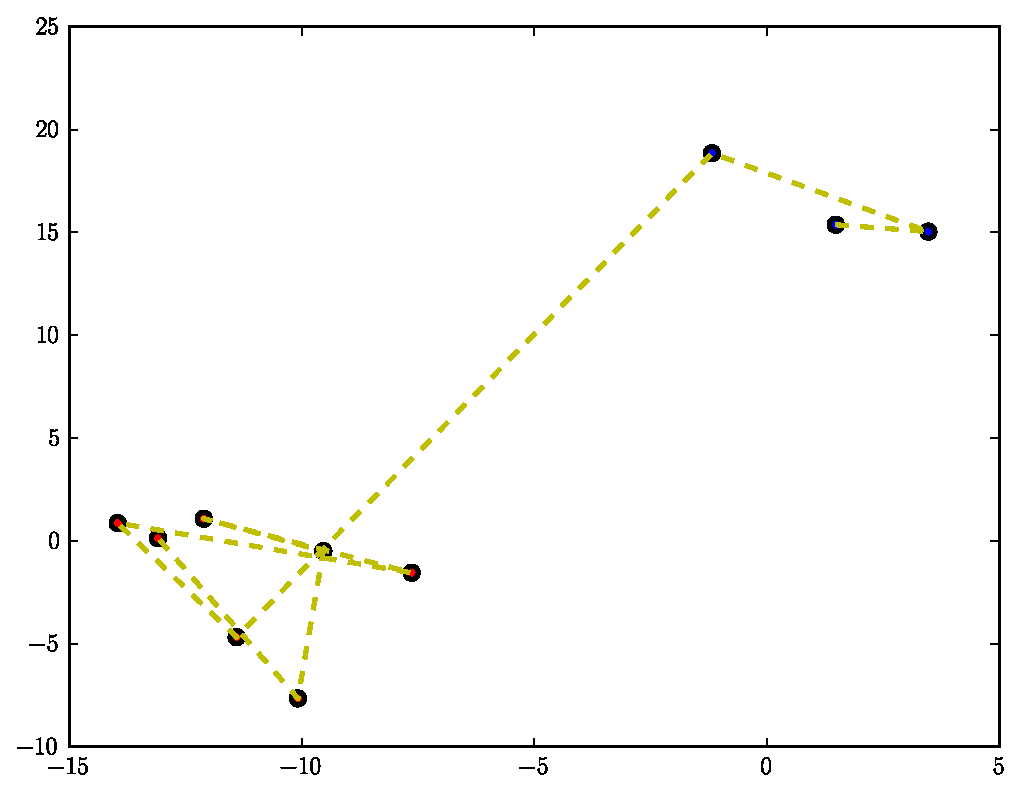
\includegraphics[width=\textwidth]{figures/samples.pdf}
\caption{Samples from the Metropolis algorithm.}
\end{figure}

\begin{problem}
Using $\mu$ and $\Sigma$ as defined previously and using an initial state $\mathbf{x} = \left[ \begin{array}{cc} 1000 & -1000 \end{array} \right]$ run your Metropolis sampler for $10000$ iterations. Plot the log probs as well as the samples. How long did it take to converge?
\end{problem}
\end{comment}

\begin{problem}
Write a function that uses the Metropolis Hastings algorithm to draw from the posterior distribution over the mean $\mu$ and variance $\sigma^2$. Use the given functions and algorithm \ref{alg:metropolis} to complete the problem.

	Your function should return an array of draws, an array of the log probabilities, and an acceptance rate. Use the following code to check your work. Using the seaborn.kdeplot function, plot the first 500 log probabilities, the $\mu$ samples and posterior distribution, and the $\sigma^2$ samples and posterior distribution. The results should be \textit{similar} to Figures \ref{fig:logprobs} and \ref{fig:metropolis_results}.

When comparing \texttt{a} to the acceptance, remember to use \texttt{log(a)} as we are in log space.


\begin{lstlisting}
# Load in the data and initialize hyperparameters.
>>> scores = np.load("examscores.npy")

# Prior sigma^2 ~ IG(alpha, beta)
>>> alpha = 3
>>> beta = 50

#Prior mu ~ N(m, s)
>>> m = 80
>>> s = 4

# Initialize the prior distributions.
>>> muprior = stats.norm(loc=m, scale=sqrt(s**2))
>>> sig2prior = stats.invgamma(alpha, scale=beta)
\end{lstlisting}

\end{problem}

\section*{The Ising Model}
In statistical mechanics, the Ising model describes how atoms interact in ferromagnetic material. Assume we have some lattice $\Lambda$ of sites. We say $i \sim j$ if $i$ and $j$ are adjacent sites. Each site $i$ in our lattice is assigned an associated \emph{spin} $\sigma_{i} \in \{\pm 1\}$. A \emph{state} in our Ising model is a particular spin configuration $\sigma = (\sigma_{k})_{k \in \Lambda}$. If $L = |\Lambda|$, then there are $2^{L}$ possible states in our model. If $L$ is large, the state space becomes huge, which is why MCMC sampling methods (in particular the Metropolis algorithm) are so useful in calculating model estimations.

With any spin configuration $\sigma$, there is an associated energy
\[
H(\sigma) = -J \sum_{i \sim j} \sigma_{i} \sigma_{j}
\]
 where $J > 0$ for ferromagnetic materials, and $J < 0$ for antiferromagnetic materials. Throughout this lab, we will assume $J = 1$, leaving the energy equation to be $H(\sigma) = -\sum_{i \sim j} \sigma_{i}\sigma_{j}$ where the interaction from each pair is added only once.

We will consider a lattice that is a $100 \times 100$ square grid.
The adjacent sites for a given site are those directly above, below, to the left, and to the right of the site, so to speak.
For sites on the edge of the grid, we assume it wraps around.
In other words, a site at the farthest left side of the grid is adjacent to the corresponding site on the farthest right side.
Thus, a single spin configuration can be represented as a $100 \times 100$ array, with entries of $\pm 1$.

The following code will construct a random spin configuration of size n:

\begin{lstlisting}
def random_lattice(n):
    """Constructs a random spin configuration for an nxn lattice."""
    random_spin = np.zeros((n,n))
    for k in range(n):
        random_spin[k,:] = 2*np.random.binomial(1,.5, n) -1
    return random_spin
\end{lstlisting}

\begin{figure}[H]
\centering
\includegraphics[width=.5\textwidth]{figures/initial_config.pdf}
\caption{Spin configuration from random initialization.}
\label{fig:random_spin}
\end{figure}

\begin{problem} % Calculate the energy of the spin configuration.
\label{problem2}
Write a function that accepts a spin configuration $\sigma$ for a lattice as a NumPy array.
Compute the energy $H(\sigma)$ of the spin configuration.
Be careful to not double count site pair interactions!
\\(Hint: \li{np.roll()} may be helpful.)
\end{problem}

Different spin configurations occur with different probabilities, depending on the energy of the spin configuration and $\beta > 0$, a quantity inversely proportional to the temperature.
More specifically, for a given $\beta$, we have
\begin{equation*}
\mathbb{P}_{\beta}(\sigma) = \frac{e^{-\beta H(\sigma)}}{Z_{\beta}}
\end{equation*}
where $Z_{\beta} = \sum_{\sigma} e^{-\beta H(\sigma)}$.
Because there are $2^{100 \cdot 100} = 2^{10000}$ possible spin configurations for our particular lattice, computing this sum is infeasible.
However, the numerator is quite simple, provided we can efficiently compute the energy $H(\sigma)$ of a spin configuration.
Thus the ratio of the probability densities of two spin configurations is simple:
\begin{equation*}
\frac{\mathbb{P}_{\beta}(\sigma^{*})}{\mathbb{P}_{\beta}(\sigma)}
= \frac{e^{-\beta H(\sigma^{*})}}{e^{-\beta H(\sigma)}}
= e^{\beta (H(\sigma) - H(\sigma^{*}))}
\end{equation*}

The simplicity of this ratio should lead us to think that a Metropolis algorithm might be an appropriate way by which to sample from the spin configuration probability distribution, in which case the acceptance probability would be
\begin{equation}
A(\sigma^{*}, \sigma) = \begin{cases} 1 & \mbox{if } H(\sigma^{*}) < H(\sigma) \\ e^{\beta (H(\sigma) - H(\sigma^{*}))} & \mbox{ otherwise.} \end{cases}
\label{eq:ising-acceptance}
\end{equation}

By choosing our transition matrix $Q$ cleverly, we can also make it easy to compute the energy for any proposed spin configuration.
We restrict our possible proposals to only those spin configurations in which we have flipped the spin at exactly one lattice site, i.e. we choose a lattice site $i$ and flip its spin.
Thus, there are only $L$ possible proposal spin configurations $\sigma^{*}$ given $\sigma$, each being proposed with probability $\frac{1}{L}$, and such that $\sigma_{j}^{*} = \sigma_{j}$ for all $j \neq i$, and $\sigma_{i}^{*} = - \sigma_{i}$.
Note that we would never actually write out this matrix (it would be $2^{10000} \times 2^{10000}$).
Computing the proposed site's energy is simple: if the spin flip site is $i$, then we have
\begin{equation}
H(\sigma^{*}) = H(\sigma) + 2\sum_{j: j \sim i} \sigma_{i}\sigma_{j}.
\label{eq:ising-new-spin-energy}
\end{equation}

\begin{problem} % Choose somewhere to flip a bit.
Write a function that accepts an integer $n$ and chooses a pair of indices $(i,j)$ where $0 \le i,j \le n-1$.
Each possible pair should have an equal probability $\frac{1}{n^2}$ of being chosen.
\label{prob:ising-flip-site}
\end{problem}

\begin{problem} % Compute the energy of the proposed configuration.
Write a function that accepts a spin configuration $\sigma$, its energy $H(\sigma)$, and integer indices $i$ and $j$.
Use \eqref{eq:ising-new-spin-energy} to compute the energy of the new spin configuration $\sigma^*$, which is $\sigma$ but with the spin flipped at the $(i,j)$th entry of the corresponding lattice.
Do not explicitly construct the new lattice for $\sigma^*$.
\label{prob:ising-new-energy}
\end{problem}

\begin{problem} % Accept / reject the new configuration.
Write a function that accepts a float $\beta$ and spin configuration energies $H(\sigma)$ and $H(\sigma^*)$.
Using \eqref{eq:ising-acceptance}, calculate whether or not the new spin configuration $\sigma^*$ should be accepted (return \li{True} or \li{False}).
Consider doing the calculations in log space.
(Hint: np.random.binomial() might be useful)
\label{prob:ising-acceptance}
\end{problem}

To track the convergence of the Markov chain, we would like to look at the probabilities of each sample at each time. However, this would require us to compute the denominator $Z_{\beta}$, which is generally the reason we have to use a Metropolis algorithm to begin with.
We can get away with examining only $-\beta H(\sigma)$.
We should see this value increase as the algorithm proceeds, and it should converge once we are sampling from the correct distribution.
Note that we don't expect these values to converge to a specific value, but rather to a restricted range of values.

\begin{problem}
Write a function that accepts a float $\beta>0$ and integers $n$, \li{n_samples}, and \li{burn_in}.
Initialize an $n\times n$ lattice for a spin configuration $\sigma$ using Problem \ref{problem2}.
Use the Metropolis algorithm to (potentially) update the lattice \li{burn_in} times.
\begin{enumerate}
    \item Use Problem \ref{prob:ising-flip-site} to choose a site for possibly flipping the spin, thus defining a potential new configuration $\sigma^*$.
    \item Use Problem \ref{prob:ising-new-energy} to calculate the energy $H(\sigma^*)$ of the proposed configuration.
    \item Use Problem \ref{prob:ising-acceptance} to accept or reject the proposed configuration.
    If it is accepted, set $\sigma = \sigma^*$ by flipping the spin at the indicated site.
    \item Track $-\beta H(\sigma)$ at each iteration (independent of acceptance).
\end{enumerate}
After the burn-in period, continue the iteration \li{n_samples} times, also recording every $100$th sample (to prevent memory failure).
The acceptance rate is counted after the burn-in period.
Return the samples, the sequence of weighted energies $-\beta H(\sigma)$, and the acceptance rate.

Test your sampler on a $100 \times 100$ grid with $200000$ total iterations, with \li{n_samples} large enough so that you will keep $50$ samples, for $\beta = 0.2, 0.4, 1$.
Plot the proportional log probabilities, as well as a late sample from each test.
How does the ferromagnetic material behave differently with differing temperatures?
Recall that $\beta$ is an inverse function of temperature.
You should see more structure with lower temperature, as illustrated in Figure \ref{fig:ising-results}.

To show the spin configuration, use \li{plt.imshow(L,cmap='gray')}.
\end{problem}

\begin{figure}
\begin{subfigure}{.49\textwidth}
    \centering
    \includegraphics[width=\textwidth]{figures/beta0_2_logprobs.pdf}
    \caption{Proportional log probs when $\beta = 0.2$.}
\end{subfigure}
%
\begin{subfigure}{.49\textwidth}
    \centering
    \includegraphics[width=.62\textwidth]{figures/beta0_2.pdf}
    \caption{Spin configuration sample when $\beta = 0.2$.}
\end{subfigure}
\\
\begin{subfigure}{.49\textwidth}
    \centering
    \includegraphics[width=\textwidth]{figures/beta0_4_logprobs.pdf}
    \caption{Proportional log probs when $\beta = 0.4$.}
\end{subfigure}
%
\begin{subfigure}{.49\textwidth}
    \centering
    \includegraphics[width=.62\textwidth]{figures/beta0_4.pdf}
        \caption{Spin configuration sample when $\beta = 0.4$.}
\end{subfigure}
\\
\begin{subfigure}{.49\textwidth}
    \centering
    \includegraphics[width=\textwidth]{figures/beta1_logprobs.pdf}
    \caption{Proportional log probs when $\beta = 1$.}
\end{subfigure}
%
\begin{subfigure}{.49\textwidth}
    \centering
    \includegraphics[width=.62\textwidth]{figures/beta1.pdf}
    \caption{Spin configuration sample when $\beta = 1$.}
\end{subfigure}
\caption{}
\label{fig:ising-results}
\end{figure}
